\chapter{Hardware Documentation and Schematics}
\label{app:hardware}

\section{Tested Board}

The manufactured V1.0 PCB was used for bring-up and testing, including rework and the final external series inductors. The drawings below show those connections and the later V1.1 changes. V1.1 was a drawing revision, not a separate manufactured test board.

\begin{table}[htbp]
\centering
\caption{Tested hardware and schematic revisions.}
\label{tab:app-revision-register}
\begin{tabularx}{\textwidth}{@{}L{0.27\textwidth}Y@{}}
\toprule
Item & Description\\
\midrule
Manufactured V1.0 PCB & Board used for prototype bring-up and final tests\\
Schematic V1.0 & Original circuit drawing\\
Schematic V1.1 & Later corrections and part changes; these were not all confirmed on the tested board\\
Earlier V2 schematic & Earlier V2 circuit drawing\\
V2 schematic and PCB & Four-sheet schematic and 31-page PCB print set; reproduced in Section~\ref{sec:app-v2-oct27}\\
Final resonant inductors & Two Wurth 7443640470B \SI{4.7}{\micro\henry} inductors in series\\
Controller & STM32G071RBT6 and the final voltage-control firmware\\
Planar magnetics & Supplied inductor and transformer assemblies from earlier DTU work\\
\bottomrule
\end{tabularx}
\end{table}

\begin{table}[htbp]
\centering
\caption{Main circuits and MCU pins on the original prototype.}
\label{tab:app-hw-anchors}
\begin{tabularx}{\textwidth}{@{}L{0.27\textwidth}Y@{}}
\toprule
Function & Component or MCU pins\\
\midrule
Switching stage & LMG2652RFBR integrated GaN half bridge\\
Output stage & MPQ4242GVE-0000-AEC1-P circuit and USB-C output path\\
Auxiliary power & BAC1S12SC and LMR54410 supply circuits\\
Sensing & Primary-voltage, secondary-voltage, and half-bridge-current paths, including AMC0330 isolation\\
Digital control & PA8/PA9 carrier; PA10 enable; PA0/PA1/PA2 analog feedback\\
\bottomrule
\end{tabularx}
\end{table}

\begin{table}[htbp]
\centering
\caption{Schematic changes from V1.0 to V1.1.}
\label{tab:app-v10-identity-card}
\small
\begin{tabularx}{\textwidth}{@{}L{0.18\textwidth}L{0.34\textwidth}Y@{}}
\toprule
Item & V1.0 drawing & V1.1 drawing\\
\midrule
C25 & \SI{22}{\micro\farad} & \SI{10}{\micro\farad}\\
Input L2 & Common-mode 7448680200 & Single \SI{100}{\micro\henry} 7447480101\\
D4--D10 & RFN1LAM6STR & PU1JLWH\\
L4 & 744778122 & 74439346082\\
MCU control & Original timer-pin assignment & Revised carrier-pin documentation\\
\bottomrule
\end{tabularx}
\end{table}

\clearpage
\section{PCB Reference Views}
\begin{figure}[htbp]
\centering
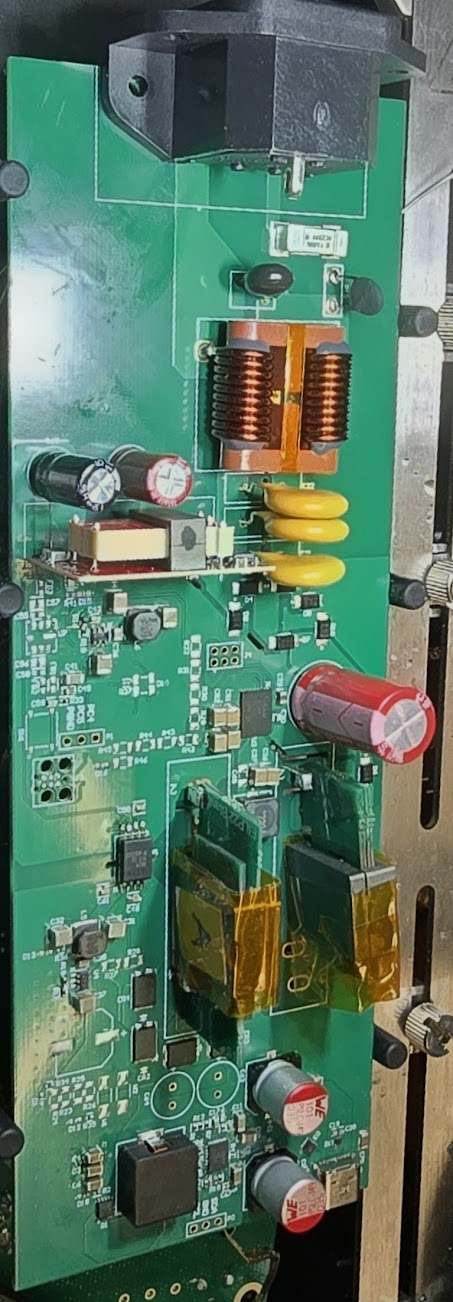
\includegraphics[height=0.49\textheight,width=\linewidth,keepaspectratio]{Pictures/Thesis/07_Hardware/final_prototype_main_photo.png}
\caption{Assembled V1.0 prototype used during final testing.}
\label{fig:app-final-prototype-photo}
\end{figure}

\begin{figure}[htbp]
\centering
\begin{subfigure}[t]{0.48\linewidth}
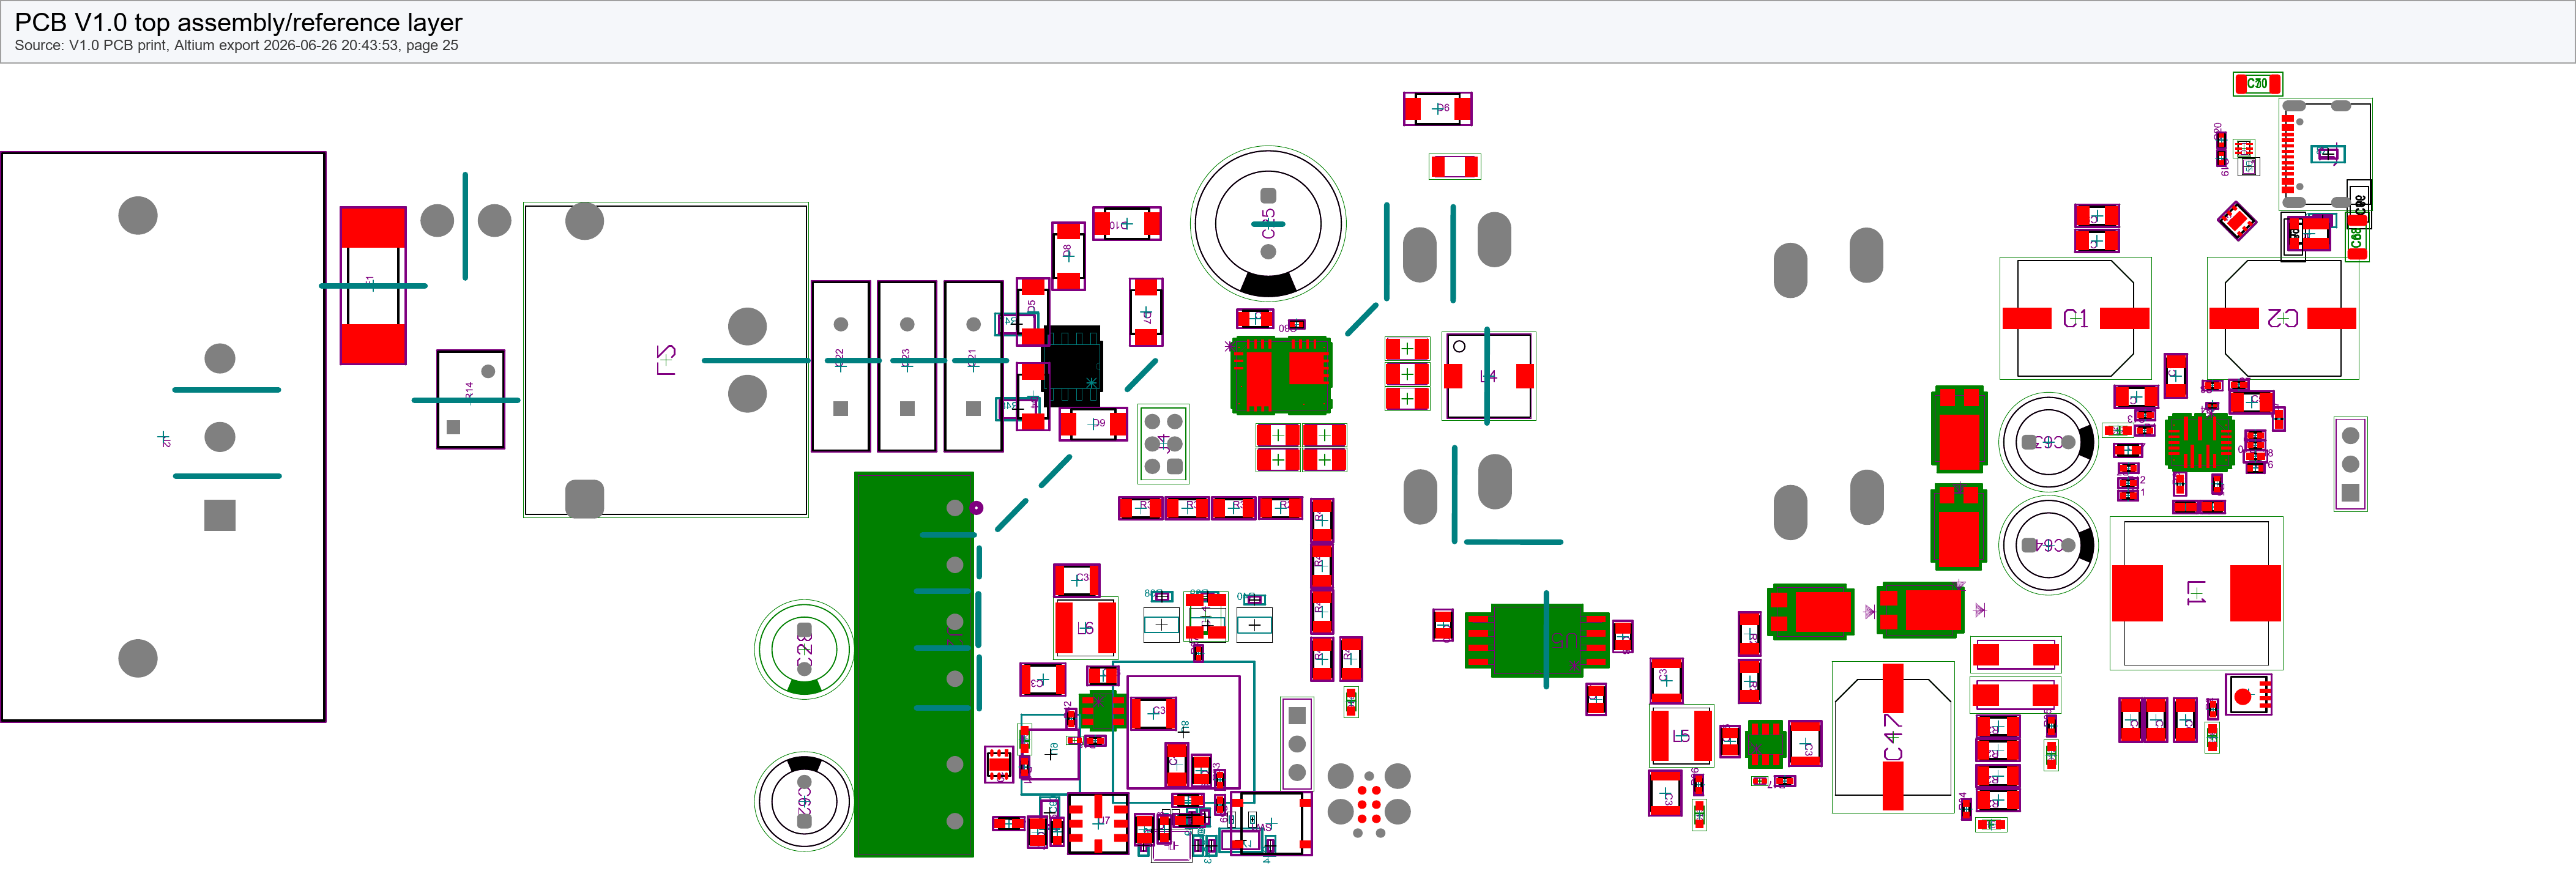
\includegraphics[width=\linewidth]{Pictures/Thesis/07_Hardware/pcb_v1_0_top_assembly_reference.png}
\caption{Assembly reference.}\label{fig:app-v10-top-reference}
\end{subfigure}\hfill
\begin{subfigure}[t]{0.48\linewidth}
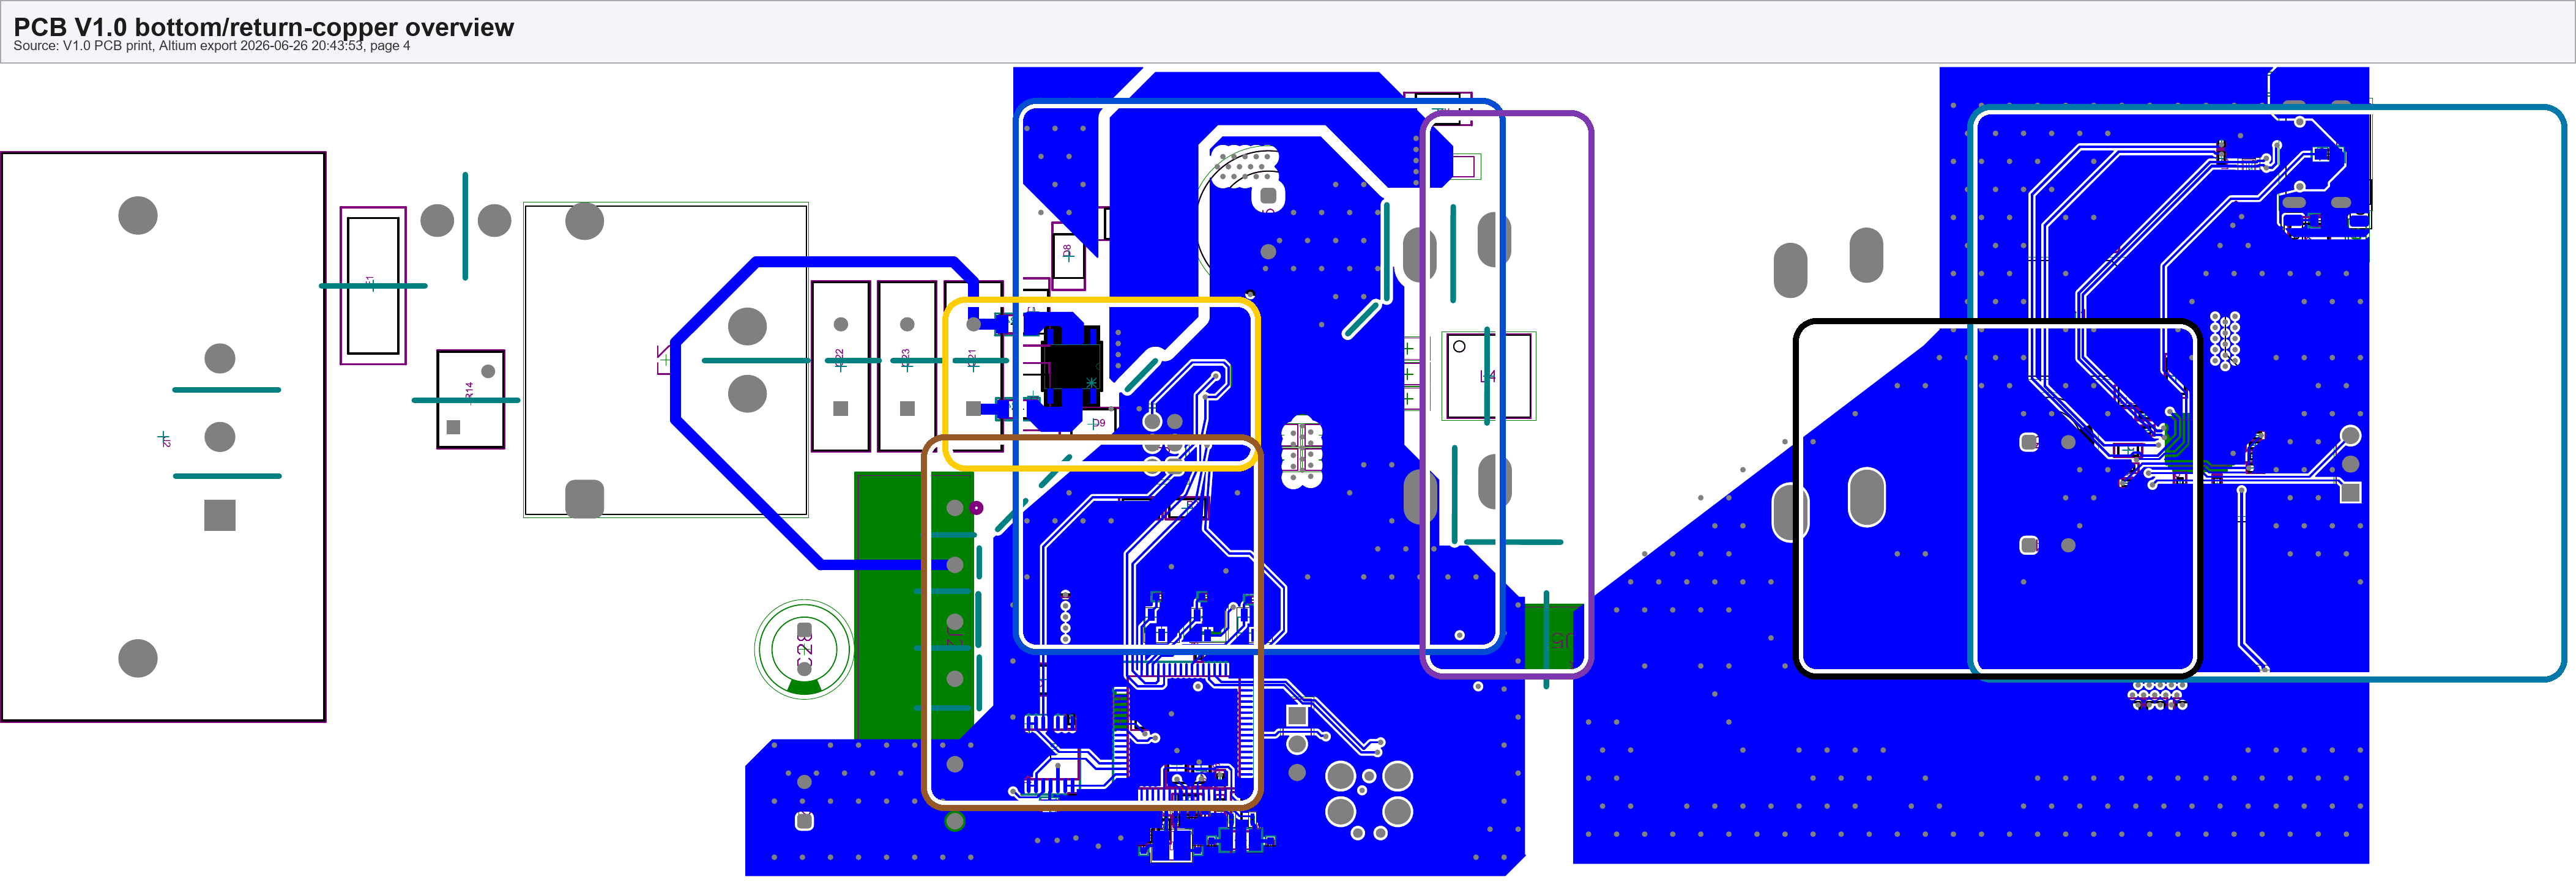
\includegraphics[width=\linewidth]{Pictures/Thesis/07_Hardware/pcb_v1_0_bottom_return_overview.png}
\caption{Bottom routing.}\label{fig:app-v10-bottom-reference}
\end{subfigure}
\caption{V1.0 PCB documentation.}\label{fig:app-v10-reference-images}
\end{figure}
\FloatBarrier

\section{Complete Schematics}
The schematic sets below cover V1.0, V1.1, and an earlier V2 circuit drawing. The complete V2 schematic and PCB design follow in Section~\ref{sec:app-v2-oct27} and support the hardware description in \cref{sec:hw-v2}. V1.0 was used for the manufactured test board; V1.1 contains the later corrections listed above. Each set contains the project hierarchy, USB-C output, power and sensing circuits, and MCU.
\clearpage\begin{landscape}
\begin{figure}[H]\centering
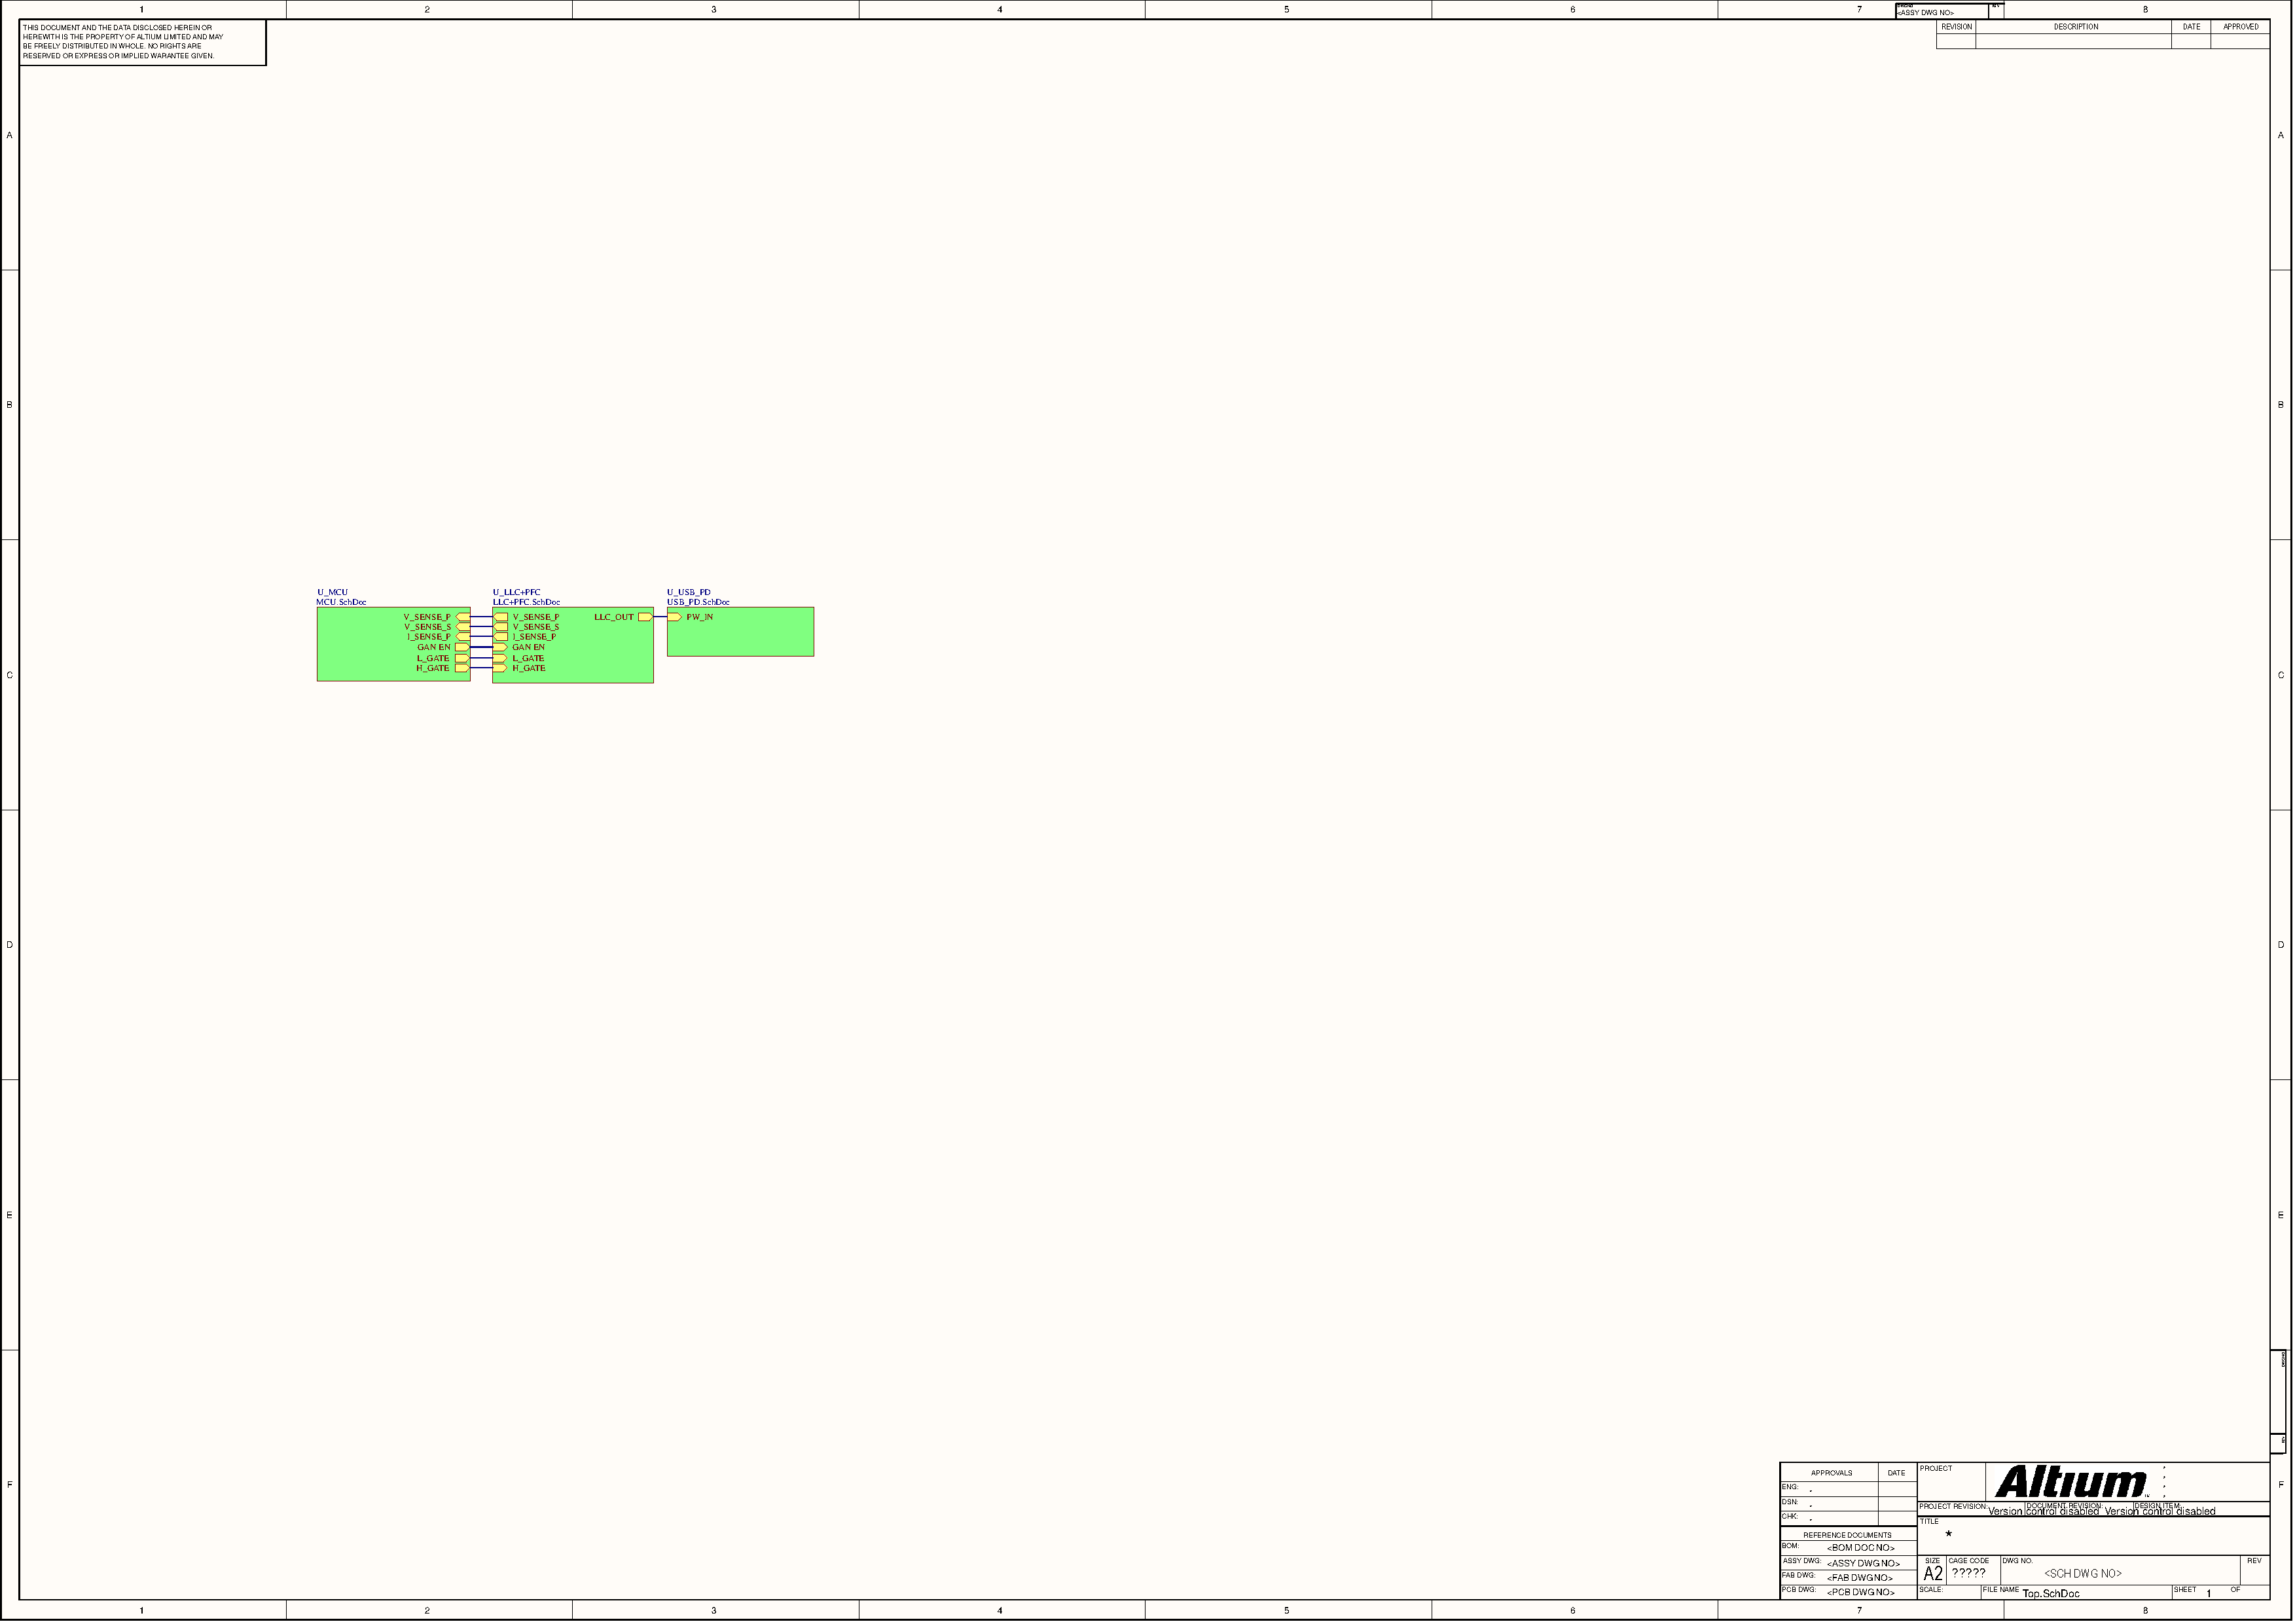
\includegraphics[page=1,width=\linewidth,height=0.86\textheight,keepaspectratio]{Pictures/Thesis/07_Hardware/Schematic_V1_0.pdf}
\caption{Schematic V1.0, sheet 1: Project hierarchy.}\label{fig:app-schematic-v10-sheet1}
\end{figure}\end{landscape}
\clearpage\begin{landscape}
\begin{figure}[H]\centering
\includegraphics[page=2,width=\linewidth,height=0.86\textheight,keepaspectratio]{Pictures/Thesis/07_Hardware/Schematic_V1_0.pdf}
\caption{Schematic V1.0, sheet 2: USB-C output stage.}\label{fig:app-schematic-v10-sheet2}
\end{figure}\end{landscape}
\clearpage\begin{landscape}
\begin{figure}[H]\centering
\includegraphics[page=3,width=\linewidth,height=0.86\textheight,keepaspectratio]{Pictures/Thesis/07_Hardware/Schematic_V1_0.pdf}
\caption{Schematic V1.0, sheet 3: Power stage, sensing, and auxiliary supplies.}\label{fig:app-schematic-v10-sheet3}
\end{figure}\end{landscape}
\clearpage\begin{landscape}
\begin{figure}[H]\centering
\includegraphics[page=4,width=\linewidth,height=0.86\textheight,keepaspectratio]{Pictures/Thesis/07_Hardware/Schematic_V1_0.pdf}
\caption{Schematic V1.0, sheet 4: MCU.}\label{fig:app-schematic-v10-sheet4}
\end{figure}\end{landscape}
\clearpage\begin{landscape}
\begin{figure}[H]\centering
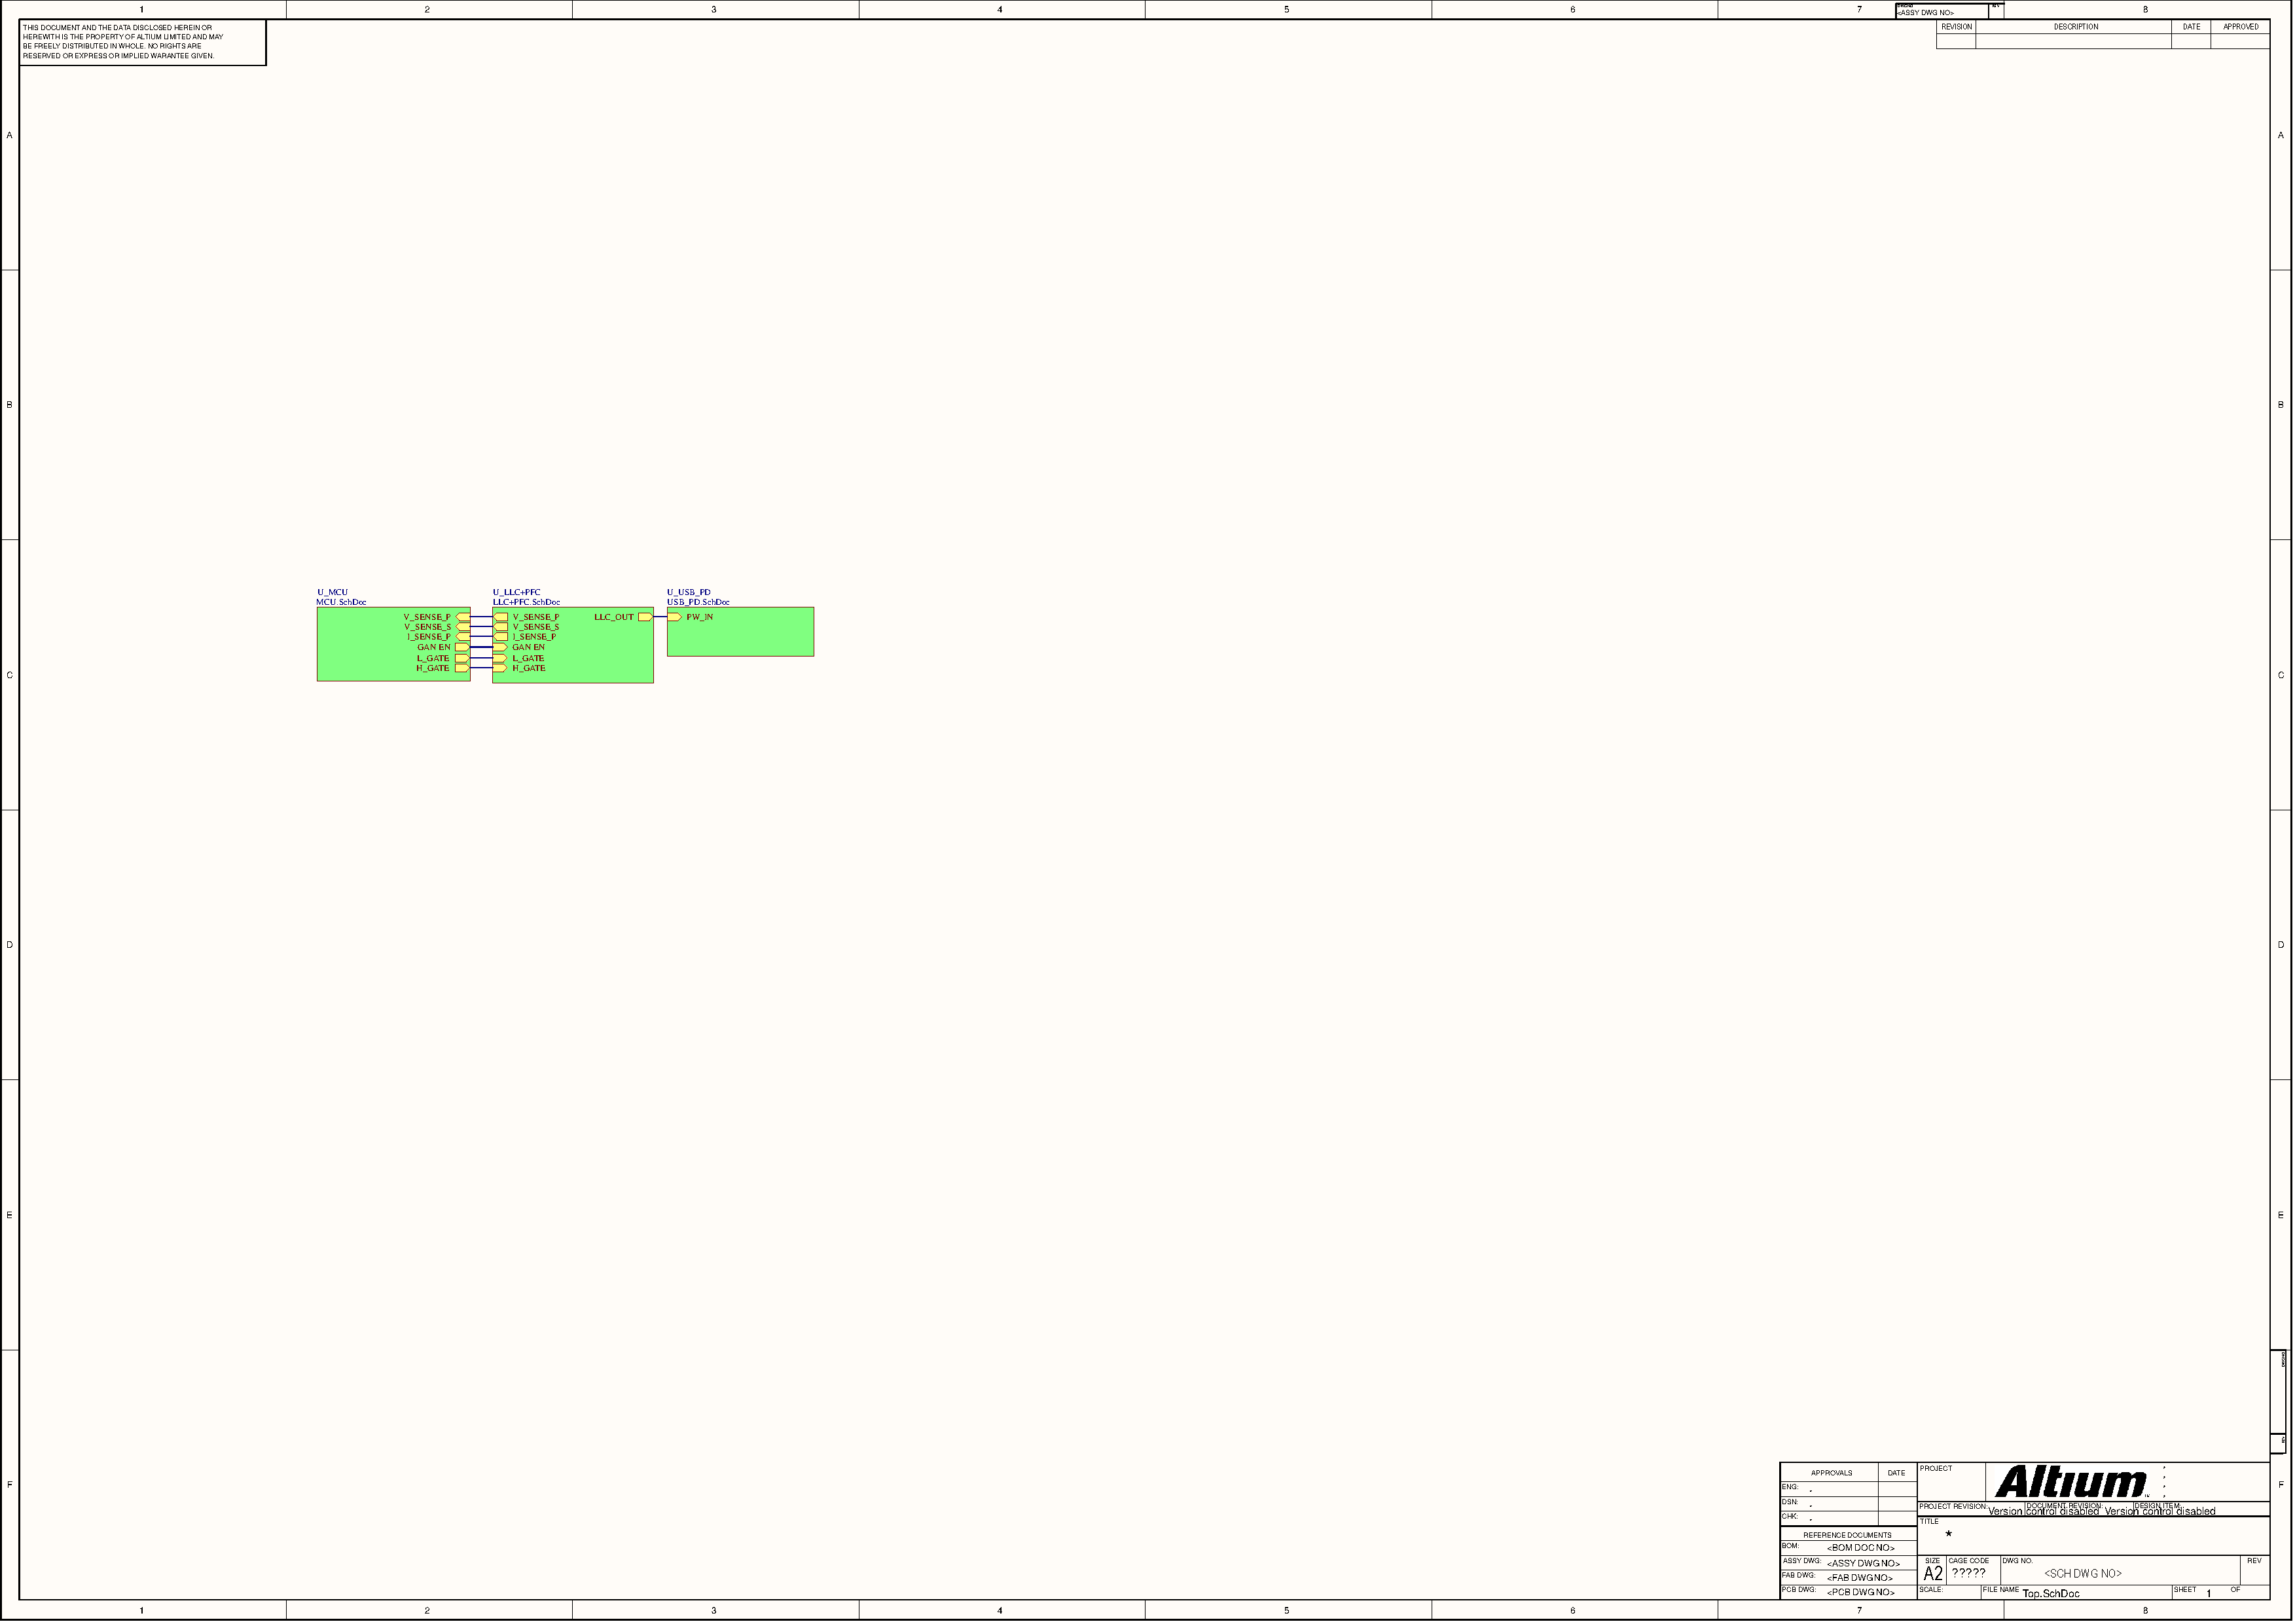
\includegraphics[page=1,width=\linewidth,height=0.86\textheight,keepaspectratio]{Pictures/Thesis/07_Hardware/Schematic_V1_1.pdf}
\caption{Schematic V1.1, sheet 1: Project hierarchy.}\label{fig:app-schematic-v11-sheet1}
\end{figure}\end{landscape}
\clearpage\begin{landscape}
\begin{figure}[H]\centering
\includegraphics[page=2,width=\linewidth,height=0.86\textheight,keepaspectratio]{Pictures/Thesis/07_Hardware/Schematic_V1_1.pdf}
\caption{Schematic V1.1, sheet 2: USB-C output stage.}\label{fig:app-schematic-v11-sheet2}
\end{figure}\end{landscape}
\clearpage\begin{landscape}
\begin{figure}[H]\centering
\includegraphics[page=3,width=\linewidth,height=0.86\textheight,keepaspectratio]{Pictures/Thesis/07_Hardware/Schematic_V1_1.pdf}
\caption{Schematic V1.1, sheet 3: Power stage, sensing, and auxiliary supplies.}\label{fig:app-schematic-v11-sheet3}
\end{figure}\end{landscape}
\clearpage\begin{landscape}
\begin{figure}[H]\centering
\includegraphics[page=4,width=\linewidth,height=0.86\textheight,keepaspectratio]{Pictures/Thesis/07_Hardware/Schematic_V1_1.pdf}
\caption{Schematic V1.1, sheet 4: MCU.}\label{fig:app-schematic-v11-sheet4}
\end{figure}\end{landscape}

\clearpage\begin{landscape}
\begin{figure}[H]\centering
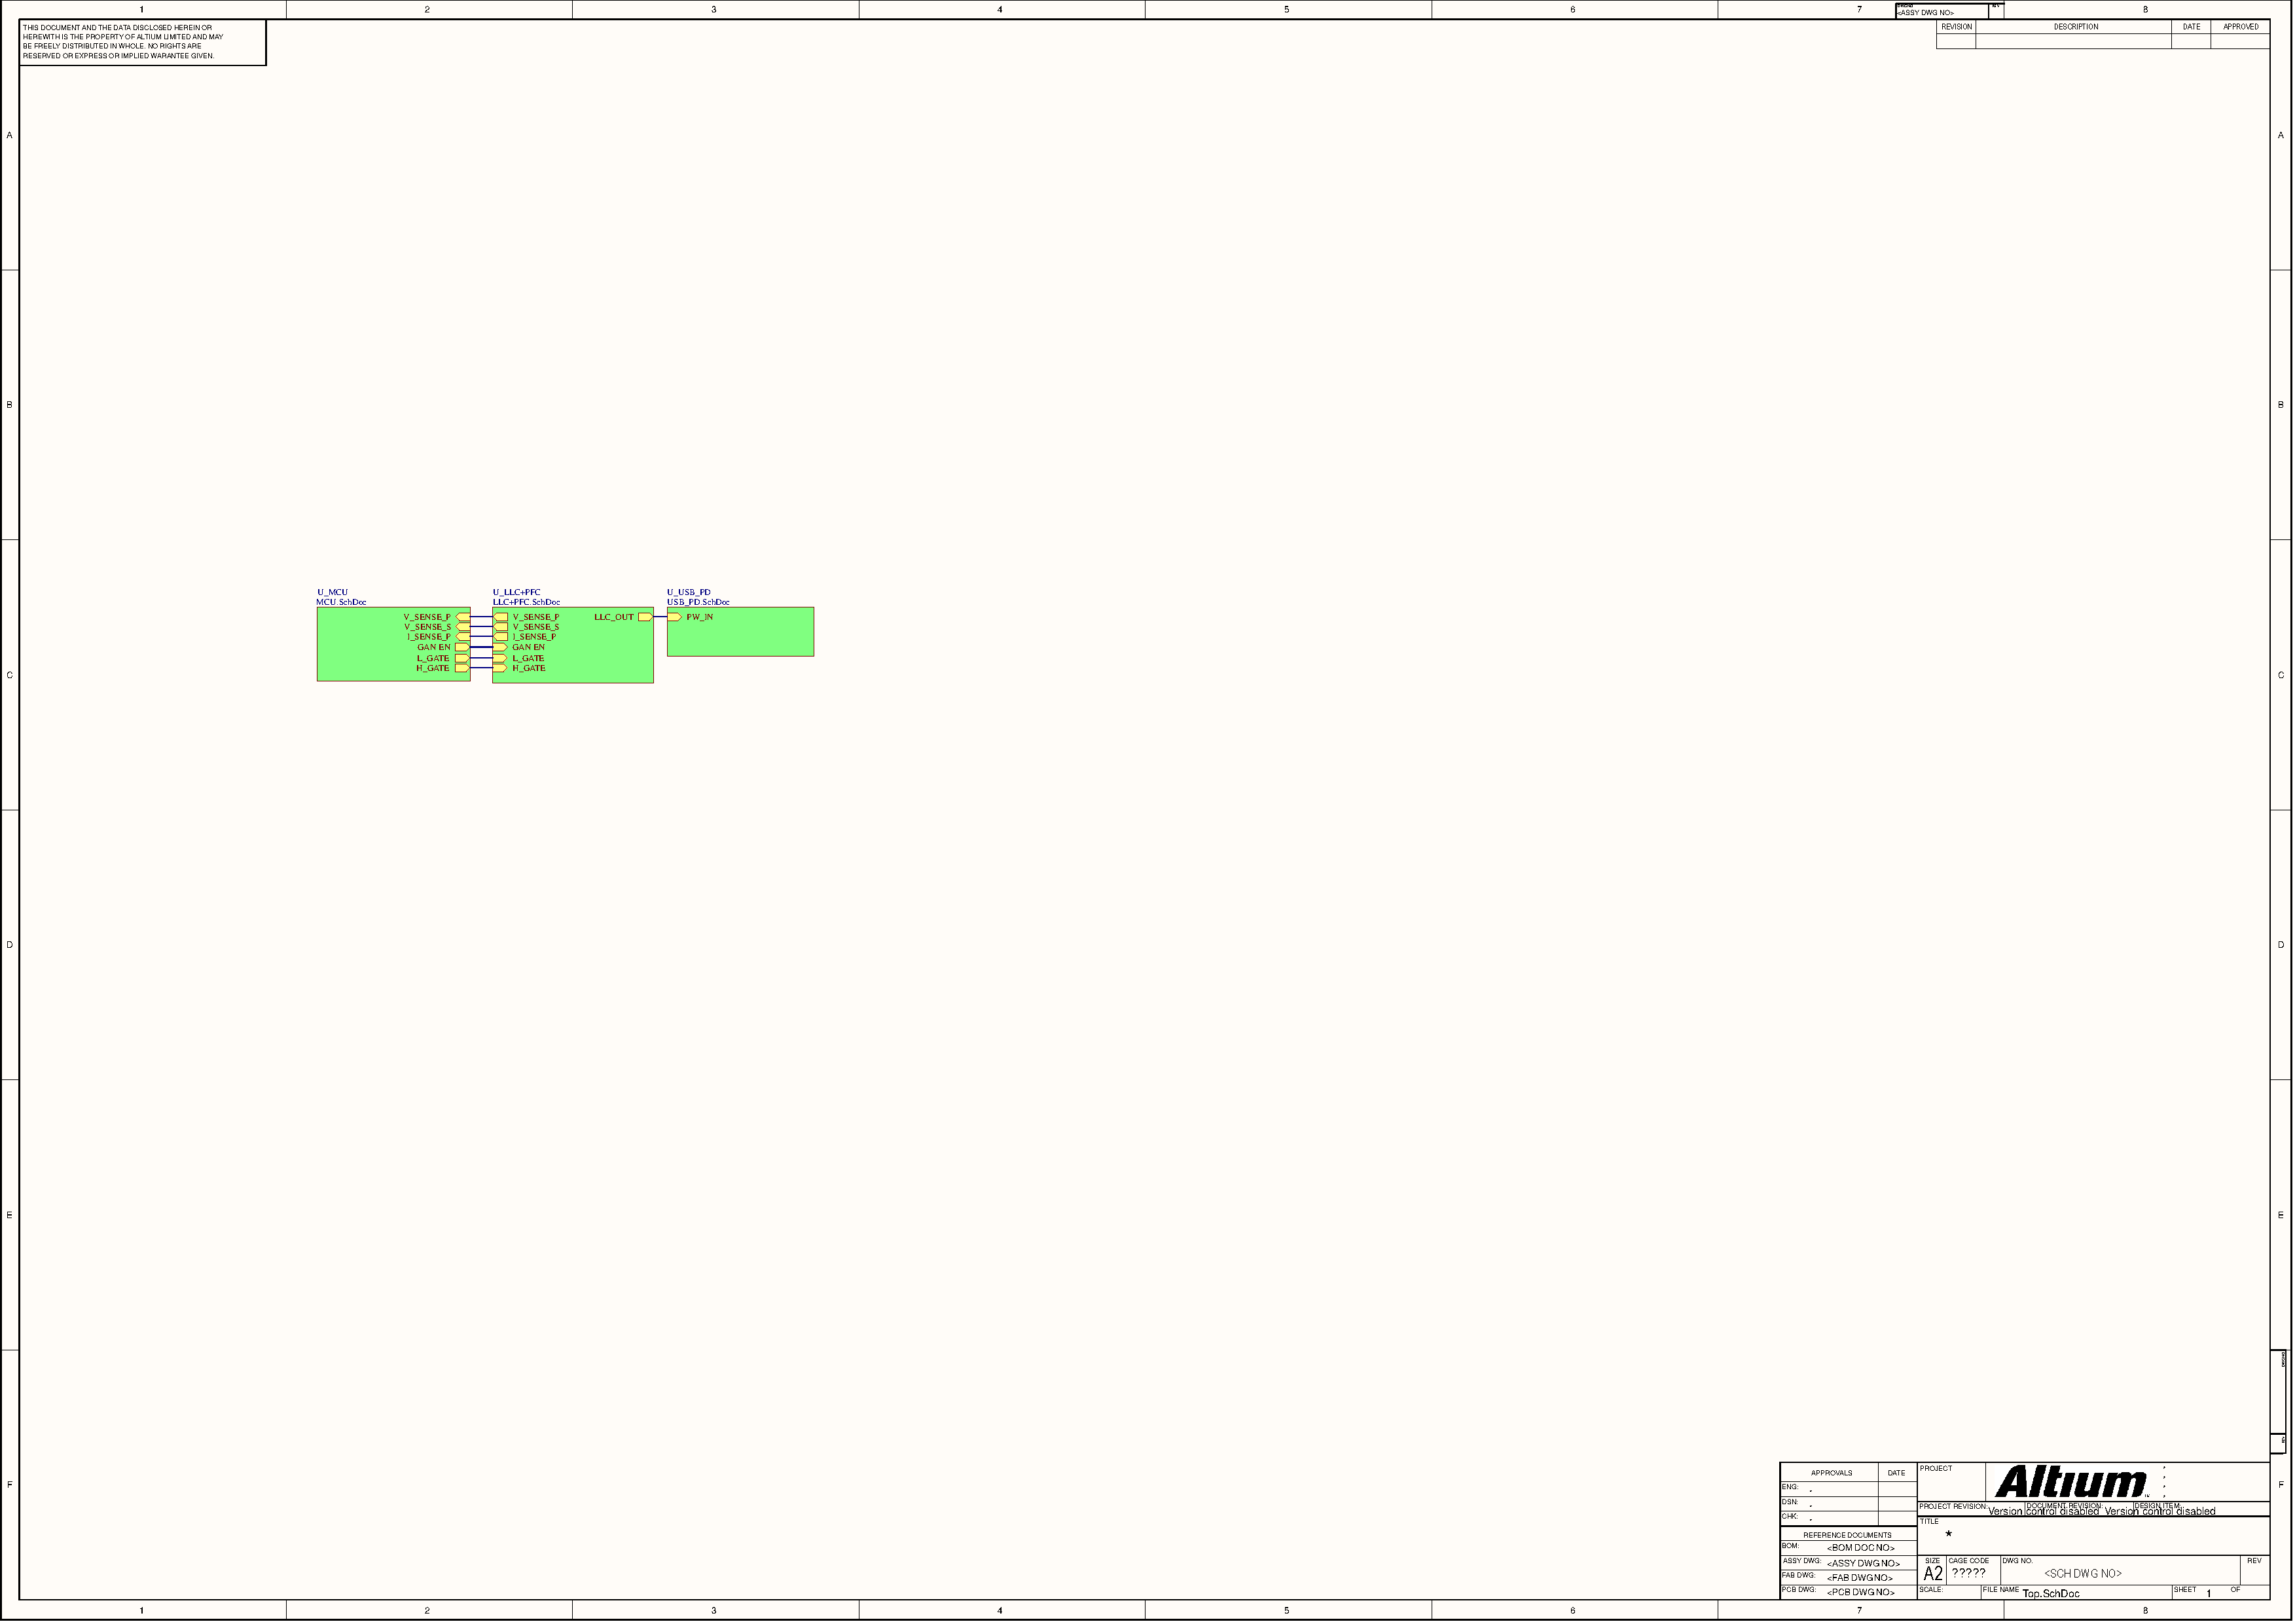
\includegraphics[page=1,width=\linewidth,height=0.86\textheight,keepaspectratio]{Pictures/Thesis/07_Hardware/Schematic_V2_F410_2026-10-18.pdf}
\caption{Earlier V2 schematic, sheet 1: Project hierarchy.}\label{fig:app-schematic-v2-sheet1}
\end{figure}\end{landscape}
\clearpage\begin{landscape}
\begin{figure}[H]\centering
\includegraphics[page=2,width=\linewidth,height=0.86\textheight,keepaspectratio]{Pictures/Thesis/07_Hardware/Schematic_V2_F410_2026-10-18.pdf}
\caption{Earlier V2 schematic, sheet 2: USB-C output stage.}\label{fig:app-schematic-v2-sheet2}
\end{figure}\end{landscape}
\clearpage\begin{landscape}
\begin{figure}[H]\centering
\includegraphics[page=3,width=\linewidth,height=0.86\textheight,keepaspectratio]{Pictures/Thesis/07_Hardware/Schematic_V2_F410_2026-10-18.pdf}
\caption{Earlier V2 schematic, sheet 3: Power stage, local supplies, and sensing (\cref{sec:hw-v2}).}\label{fig:app-schematic-v2-sheet3}
\end{figure}\end{landscape}
\clearpage\begin{landscape}
\begin{figure}[H]\centering
\includegraphics[page=4,width=\linewidth,height=0.86\textheight,keepaspectratio]{Pictures/Thesis/07_Hardware/Schematic_V2_F410_2026-10-18.pdf}
\caption{Earlier V2 schematic, sheet 4: MCU and direct PA0--PA2 feedback connections.}\label{fig:app-schematic-v2-sheet4}
\end{figure}\end{landscape}


\clearpage
\section{V2 Schematic and PCB Design}
\label{sec:app-v2-oct27}

The V2 circuit was organized around the MCU, the charge-pump/resonant
converter, and the USB-C output stage. The four-sheet schematic and
complete 31-page PCB print set are reproduced below. The component values
and feedback scaling that still need confirmation are discussed in
\cref{sec:hw-v2}.

The PCB drawings cover the top and bottom copper, two internal copper
layers, silkscreen, mask, assembly, mechanical, and drill information.
Layers named ``3D Body'' show the projected component outlines.
The drawings describe the original board design. The tank changes made
during powered testing are described in \cref{sec:res-v2-testing}.

\clearpage\begin{landscape}
\begin{figure}[H]\centering
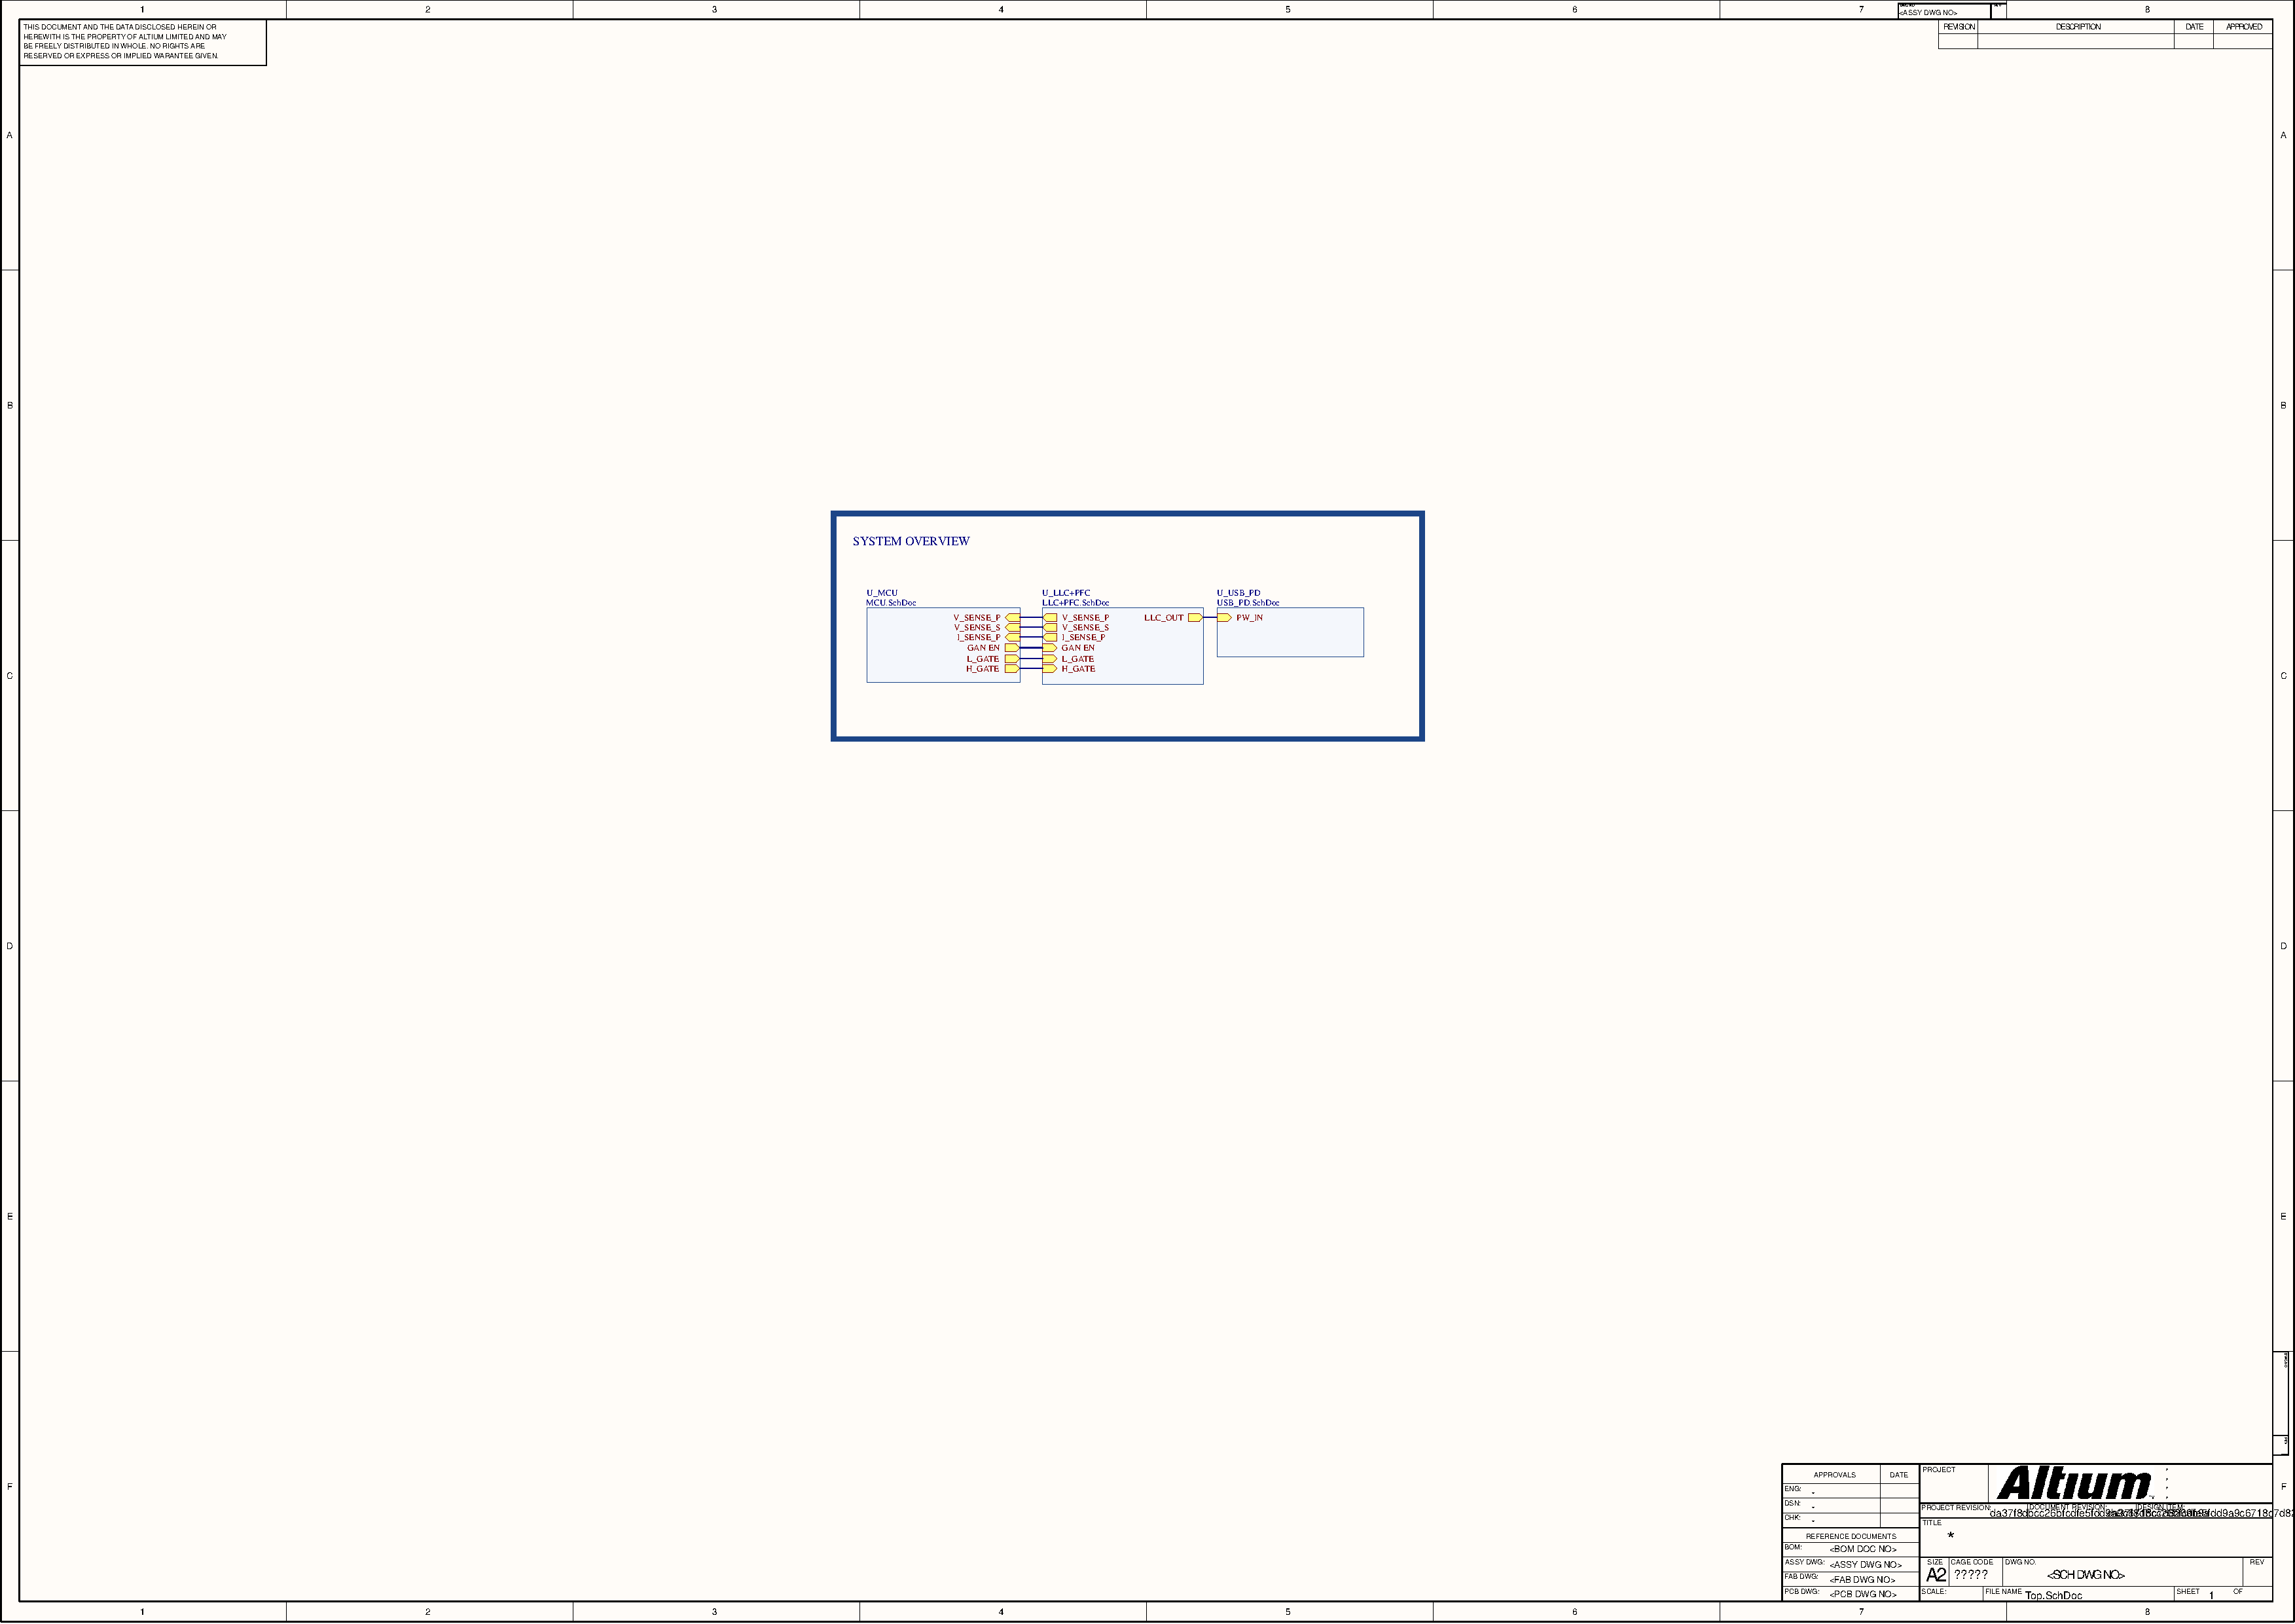
\includegraphics[page=1,width=\linewidth,height=0.86\textheight,keepaspectratio]{Pictures/Thesis/07_Hardware/Schematic_V2_Colour.pdf}
\caption{V2 schematic, sheet 1: System overview.}\label{fig:app-v2-oct27-schematic-1}
\end{figure}\end{landscape}

\clearpage\begin{landscape}
\begin{figure}[H]\centering
\includegraphics[page=2,width=\linewidth,height=0.86\textheight,keepaspectratio]{Pictures/Thesis/07_Hardware/Schematic_V2_Colour.pdf}
\caption{V2 schematic, sheet 2: USB-C output stage.}\label{fig:app-v2-oct27-schematic-2}
\end{figure}\end{landscape}

\clearpage\begin{landscape}
\begin{figure}[H]\centering
\includegraphics[page=3,width=\linewidth,height=0.86\textheight,keepaspectratio]{Pictures/Thesis/07_Hardware/Schematic_V2_Colour.pdf}
\caption{V2 schematic, sheet 3: Power stage, sensing, and local supplies.}\label{fig:app-v2-oct27-schematic-3}
\end{figure}\end{landscape}

\clearpage\begin{landscape}
\begin{figure}[H]\centering
\includegraphics[page=4,width=\linewidth,height=0.86\textheight,keepaspectratio]{Pictures/Thesis/07_Hardware/Schematic_V2_Colour.pdf}
\caption{V2 schematic, sheet 4: MCU and service connections.}\label{fig:app-v2-oct27-schematic-4}
\end{figure}\end{landscape}

\clearpage\begin{landscape}
\begin{figure}[H]\centering
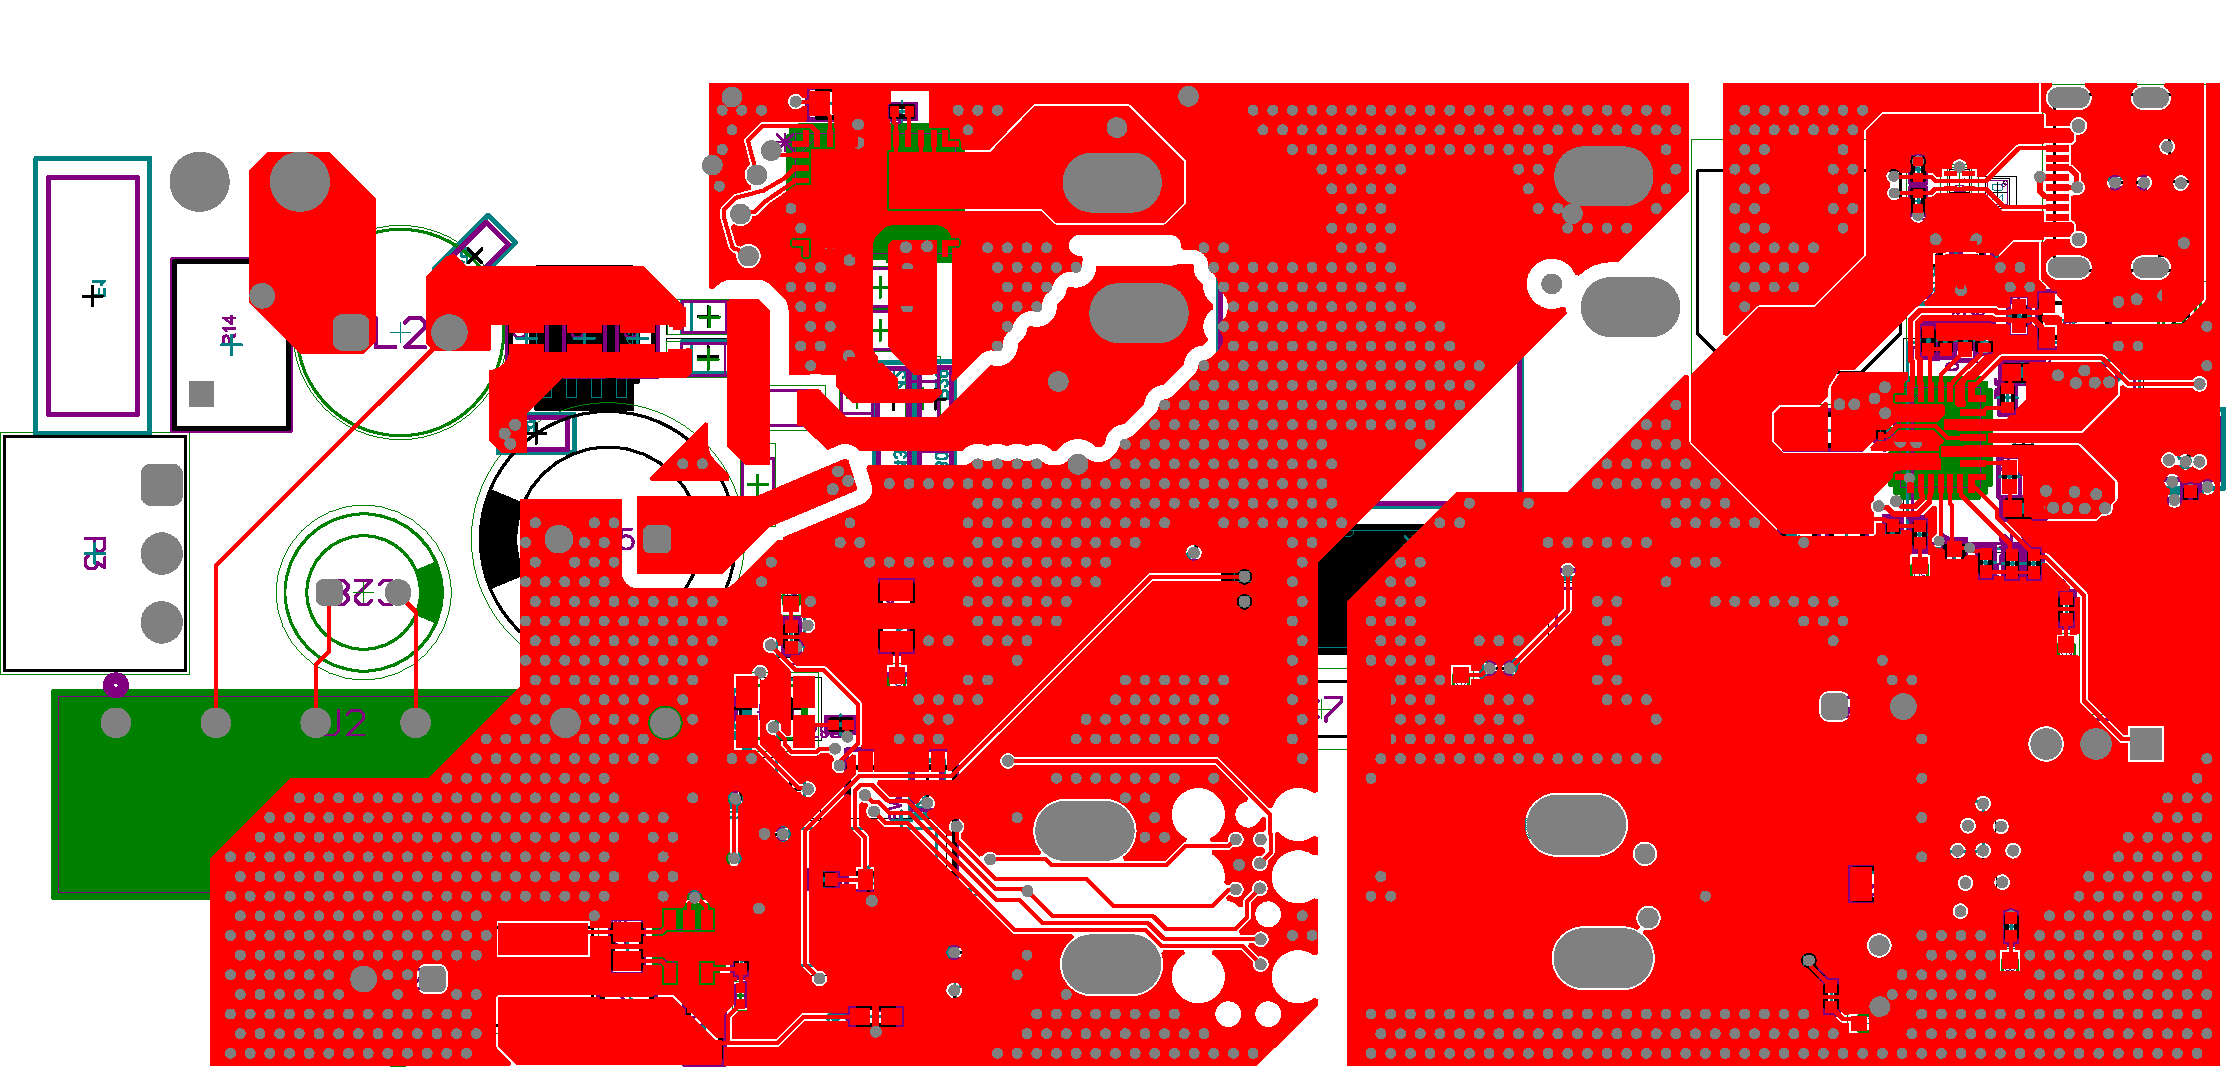
\includegraphics[page=1,width=\linewidth,height=0.86\textheight,keepaspectratio]{Pictures/Thesis/07_Hardware/PCB_V2_F410_2026-10-27.pdf}
\caption{V2 PCB print 1: Top Layer.}\label{fig:app-v2-oct27-pcb-1}
\end{figure}\end{landscape}

\clearpage\begin{landscape}
\begin{figure}[H]\centering
\includegraphics[page=2,width=\linewidth,height=0.86\textheight,keepaspectratio]{Pictures/Thesis/07_Hardware/PCB_V2_F410_2026-10-27.pdf}
\caption{V2 PCB print 2: Int1 (GND).}\label{fig:app-v2-oct27-pcb-2}
\end{figure}\end{landscape}

\clearpage\begin{landscape}
\begin{figure}[H]\centering
\includegraphics[page=3,width=\linewidth,height=0.86\textheight,keepaspectratio]{Pictures/Thesis/07_Hardware/PCB_V2_F410_2026-10-27.pdf}
\caption{V2 PCB print 3: Int2 (PWR).}\label{fig:app-v2-oct27-pcb-3}
\end{figure}\end{landscape}

\clearpage\begin{landscape}
\begin{figure}[H]\centering
\includegraphics[page=4,width=\linewidth,height=0.86\textheight,keepaspectratio]{Pictures/Thesis/07_Hardware/PCB_V2_F410_2026-10-27.pdf}
\caption{V2 PCB print 4: Bottom Layer.}\label{fig:app-v2-oct27-pcb-4}
\end{figure}\end{landscape}

\clearpage\begin{landscape}
\begin{figure}[H]\centering
\includegraphics[page=5,width=\linewidth,height=0.86\textheight,keepaspectratio]{Pictures/Thesis/07_Hardware/PCB_V2_F410_2026-10-27.pdf}
\caption{V2 PCB print 5: Top Silkscreen Overlay.}\label{fig:app-v2-oct27-pcb-5}
\end{figure}\end{landscape}

\clearpage\begin{landscape}
\begin{figure}[H]\centering
\includegraphics[page=6,width=\linewidth,height=0.86\textheight,keepaspectratio]{Pictures/Thesis/07_Hardware/PCB_V2_F410_2026-10-27.pdf}
\caption{V2 PCB print 6: Bottom Silkscreen Overlay.}\label{fig:app-v2-oct27-pcb-6}
\end{figure}\end{landscape}

\clearpage\begin{landscape}
\begin{figure}[H]\centering
\includegraphics[page=7,width=\linewidth,height=0.86\textheight,keepaspectratio]{Pictures/Thesis/07_Hardware/PCB_V2_F410_2026-10-27.pdf}
\caption{V2 PCB print 7: Top Paste Mask Print.}\label{fig:app-v2-oct27-pcb-7}
\end{figure}\end{landscape}

\clearpage\begin{landscape}
\begin{figure}[H]\centering
\includegraphics[page=8,width=\linewidth,height=0.86\textheight,keepaspectratio]{Pictures/Thesis/07_Hardware/PCB_V2_F410_2026-10-27.pdf}
\caption{V2 PCB print 8: Bottom Paste Mask Print.}\label{fig:app-v2-oct27-pcb-8}
\end{figure}\end{landscape}

\clearpage\begin{landscape}
\begin{figure}[H]\centering
\includegraphics[page=9,width=\linewidth,height=0.86\textheight,keepaspectratio]{Pictures/Thesis/07_Hardware/PCB_V2_F410_2026-10-27.pdf}
\caption{V2 PCB print 9: Top Solder Mask Print.}\label{fig:app-v2-oct27-pcb-9}
\end{figure}\end{landscape}

\clearpage\begin{landscape}
\begin{figure}[H]\centering
\includegraphics[page=10,width=\linewidth,height=0.86\textheight,keepaspectratio]{Pictures/Thesis/07_Hardware/PCB_V2_F410_2026-10-27.pdf}
\caption{V2 PCB print 10: Board.}\label{fig:app-v2-oct27-pcb-10}
\end{figure}\end{landscape}

\clearpage\begin{landscape}
\begin{figure}[H]\centering
\includegraphics[page=11,width=\linewidth,height=0.86\textheight,keepaspectratio]{Pictures/Thesis/07_Hardware/PCB_V2_F410_2026-10-27.pdf}
\caption{V2 PCB print 11: Top Tenting.}\label{fig:app-v2-oct27-pcb-11}
\end{figure}\end{landscape}

\clearpage\begin{landscape}
\begin{figure}[H]\centering
\includegraphics[page=12,width=\linewidth,height=0.86\textheight,keepaspectratio]{Pictures/Thesis/07_Hardware/PCB_V2_F410_2026-10-27.pdf}
\caption{V2 PCB print 12: Bottom Tenting.}\label{fig:app-v2-oct27-pcb-12}
\end{figure}\end{landscape}

\clearpage\begin{landscape}
\begin{figure}[H]\centering
\includegraphics[page=13,width=\linewidth,height=0.86\textheight,keepaspectratio]{Pictures/Thesis/07_Hardware/PCB_V2_F410_2026-10-27.pdf}
\caption{V2 PCB print 13: Bottom Component Center.}\label{fig:app-v2-oct27-pcb-13}
\end{figure}\end{landscape}

\clearpage\begin{landscape}
\begin{figure}[H]\centering
\includegraphics[page=14,width=\linewidth,height=0.86\textheight,keepaspectratio]{Pictures/Thesis/07_Hardware/PCB_V2_F410_2026-10-27.pdf}
\caption{V2 PCB print 14: Route Tool Path.}\label{fig:app-v2-oct27-pcb-14}
\end{figure}\end{landscape}

\clearpage\begin{landscape}
\begin{figure}[H]\centering
\includegraphics[page=15,width=\linewidth,height=0.86\textheight,keepaspectratio]{Pictures/Thesis/07_Hardware/PCB_V2_F410_2026-10-27.pdf}
\caption{V2 PCB print 15: Top 3D Body.}\label{fig:app-v2-oct27-pcb-15}
\end{figure}\end{landscape}

\clearpage\begin{landscape}
\begin{figure}[H]\centering
\includegraphics[page=16,width=\linewidth,height=0.86\textheight,keepaspectratio]{Pictures/Thesis/07_Hardware/PCB_V2_F410_2026-10-27.pdf}
\caption{V2 PCB print 16: Bottom 3D Body.}\label{fig:app-v2-oct27-pcb-16}
\end{figure}\end{landscape}

\clearpage\begin{landscape}
\begin{figure}[H]\centering
\includegraphics[page=17,width=\linewidth,height=0.86\textheight,keepaspectratio]{Pictures/Thesis/07_Hardware/PCB_V2_F410_2026-10-27.pdf}
\caption{V2 PCB print 17: Top Component Center.}\label{fig:app-v2-oct27-pcb-17}
\end{figure}\end{landscape}

\clearpage\begin{landscape}
\begin{figure}[H]\centering
\includegraphics[page=18,width=\linewidth,height=0.86\textheight,keepaspectratio]{Pictures/Thesis/07_Hardware/PCB_V2_F410_2026-10-27.pdf}
\caption{V2 PCB print 18: Top Component Outline.}\label{fig:app-v2-oct27-pcb-18}
\end{figure}\end{landscape}

\clearpage\begin{landscape}
\begin{figure}[H]\centering
\includegraphics[page=19,width=\linewidth,height=0.86\textheight,keepaspectratio]{Pictures/Thesis/07_Hardware/PCB_V2_F410_2026-10-27.pdf}
\caption{V2 PCB print 19: Bottom Component Outline.}\label{fig:app-v2-oct27-pcb-19}
\end{figure}\end{landscape}

\clearpage\begin{landscape}
\begin{figure}[H]\centering
\includegraphics[page=20,width=\linewidth,height=0.86\textheight,keepaspectratio]{Pictures/Thesis/07_Hardware/PCB_V2_F410_2026-10-27.pdf}
\caption{V2 PCB print 20: Top Coating.}\label{fig:app-v2-oct27-pcb-20}
\end{figure}\end{landscape}

\clearpage\begin{landscape}
\begin{figure}[H]\centering
\includegraphics[page=21,width=\linewidth,height=0.86\textheight,keepaspectratio]{Pictures/Thesis/07_Hardware/PCB_V2_F410_2026-10-27.pdf}
\caption{V2 PCB print 21: Bottom Coating.}\label{fig:app-v2-oct27-pcb-21}
\end{figure}\end{landscape}

\clearpage\begin{landscape}
\begin{figure}[H]\centering
\includegraphics[page=22,width=\linewidth,height=0.86\textheight,keepaspectratio]{Pictures/Thesis/07_Hardware/PCB_V2_F410_2026-10-27.pdf}
\caption{V2 PCB print 22: Top Assembly.}\label{fig:app-v2-oct27-pcb-22}
\end{figure}\end{landscape}

\clearpage\begin{landscape}
\begin{figure}[H]\centering
\includegraphics[page=23,width=\linewidth,height=0.86\textheight,keepaspectratio]{Pictures/Thesis/07_Hardware/PCB_V2_F410_2026-10-27.pdf}
\caption{V2 PCB print 23: Bottom Assembly.}\label{fig:app-v2-oct27-pcb-23}
\end{figure}\end{landscape}

\clearpage\begin{landscape}
\begin{figure}[H]\centering
\includegraphics[page=24,width=\linewidth,height=0.86\textheight,keepaspectratio]{Pictures/Thesis/07_Hardware/PCB_V2_F410_2026-10-27.pdf}
\caption{V2 PCB print 24: Top Courtyard.}\label{fig:app-v2-oct27-pcb-24}
\end{figure}\end{landscape}

\clearpage\begin{landscape}
\begin{figure}[H]\centering
\includegraphics[page=25,width=\linewidth,height=0.86\textheight,keepaspectratio]{Pictures/Thesis/07_Hardware/PCB_V2_F410_2026-10-27.pdf}
\caption{V2 PCB print 25: Bottom Courtyard.}\label{fig:app-v2-oct27-pcb-25}
\end{figure}\end{landscape}

\clearpage\begin{landscape}
\begin{figure}[H]\centering
\includegraphics[page=26,width=\linewidth,height=0.86\textheight,keepaspectratio]{Pictures/Thesis/07_Hardware/PCB_V2_F410_2026-10-27.pdf}
\caption{V2 PCB print 26: Top Designator.}\label{fig:app-v2-oct27-pcb-26}
\end{figure}\end{landscape}

\clearpage\begin{landscape}
\begin{figure}[H]\centering
\includegraphics[page=27,width=\linewidth,height=0.86\textheight,keepaspectratio]{Pictures/Thesis/07_Hardware/PCB_V2_F410_2026-10-27.pdf}
\caption{V2 PCB print 27: Bottom Designator.}\label{fig:app-v2-oct27-pcb-27}
\end{figure}\end{landscape}

\clearpage\begin{landscape}
\begin{figure}[H]\centering
\includegraphics[page=28,width=\linewidth,height=0.86\textheight,keepaspectratio]{Pictures/Thesis/07_Hardware/PCB_V2_F410_2026-10-27.pdf}
\caption{V2 PCB print 28: Top Pad Master.}\label{fig:app-v2-oct27-pcb-28}
\end{figure}\end{landscape}

\clearpage\begin{landscape}
\begin{figure}[H]\centering
\includegraphics[page=29,width=\linewidth,height=0.86\textheight,keepaspectratio]{Pictures/Thesis/07_Hardware/PCB_V2_F410_2026-10-27.pdf}
\caption{V2 PCB print 29: Bottom Pad Master.}\label{fig:app-v2-oct27-pcb-29}
\end{figure}\end{landscape}

\clearpage\begin{landscape}
\begin{figure}[H]\centering
\includegraphics[page=30,width=\linewidth,height=0.86\textheight,keepaspectratio]{Pictures/Thesis/07_Hardware/PCB_V2_F410_2026-10-27.pdf}
\caption{V2 PCB print 30: Drill Drawing For (Top Layer - Bottom Layer).}\label{fig:app-v2-oct27-pcb-30}
\end{figure}\end{landscape}

\clearpage\begin{landscape}
\begin{figure}[H]\centering
\includegraphics[page=31,width=\linewidth,height=0.86\textheight,keepaspectratio]{Pictures/Thesis/07_Hardware/PCB_V2_F410_2026-10-27.pdf}
\caption{V2 PCB print 31: Drill Guide For (Top Layer - Bottom Layer).}\label{fig:app-v2-oct27-pcb-31}
\end{figure}\end{landscape}
